\section{Experimentación Y Resultados}

A continuación expondremos los resultados obtenidos por cada algoritmo para distintas imágenes. El objetivo será posteriormente hacer análisis de calidad subjetiva (es decir que vemos a simple vista), objetiva y tiempo de computos. Para, como dijimos en un principio, determinar ventajas y desventajas de cada uno de ellos. Para los análisis objetivos desarrollamos un programa en python que compara pixel a pixel basado en PSNR (Peak signal-to-noise ratio). Elegimos 3 casos particulares pero como se verá, los resultados son parecidos y se ha comportado de la misma manera en los otros ejemplos dados por la cátedra y lo mismo en otros ejemplos nuestros que no valían la pena ponerlos en el informe.

\subsection{PNSR}
Es un método para definir la relación entre una señal y el ruido de la regenaración de la misma expresado en decibeles. En este caso, así como es comunmente utilizado, sirve para resolver si la imagen final es "parecida" a la original. Es importante notar que a medida que mayor sea el resultado, mejor es la calidad de la imágen.

\subsection{Colores}


Se nos ocurrió que podría ser interesante chequear los comportamientos de estos procedimientos en una imagen con muchos bordes ya que estos, en algoritmos como el directional, son factores importantes y potencialmente conflictivos. Además hicimos que la imagen sea grande (5000 x 3000 pixeles) para poder analizar tiempos de computo y para influir en la calidad subjetiva, ya que si ponemos imágenes con mucha definición pequeños errores podrían pasar desapercividos para el ojo humano.

Tambien expondremos la imagen bayerizada para que quede claro que la conversción que estamos haciendo es correcta.

\begin{figure}

\minipage{0.5\textwidth}
\begin{center}
       
\includegraphics[scale=0.04]{imagenes/colores.png}
       \caption{Original }\label{fig:awesome_image1}
        \end{center}
\endminipage\hfill
\minipage{0.5\textwidth}
\begin{center}
        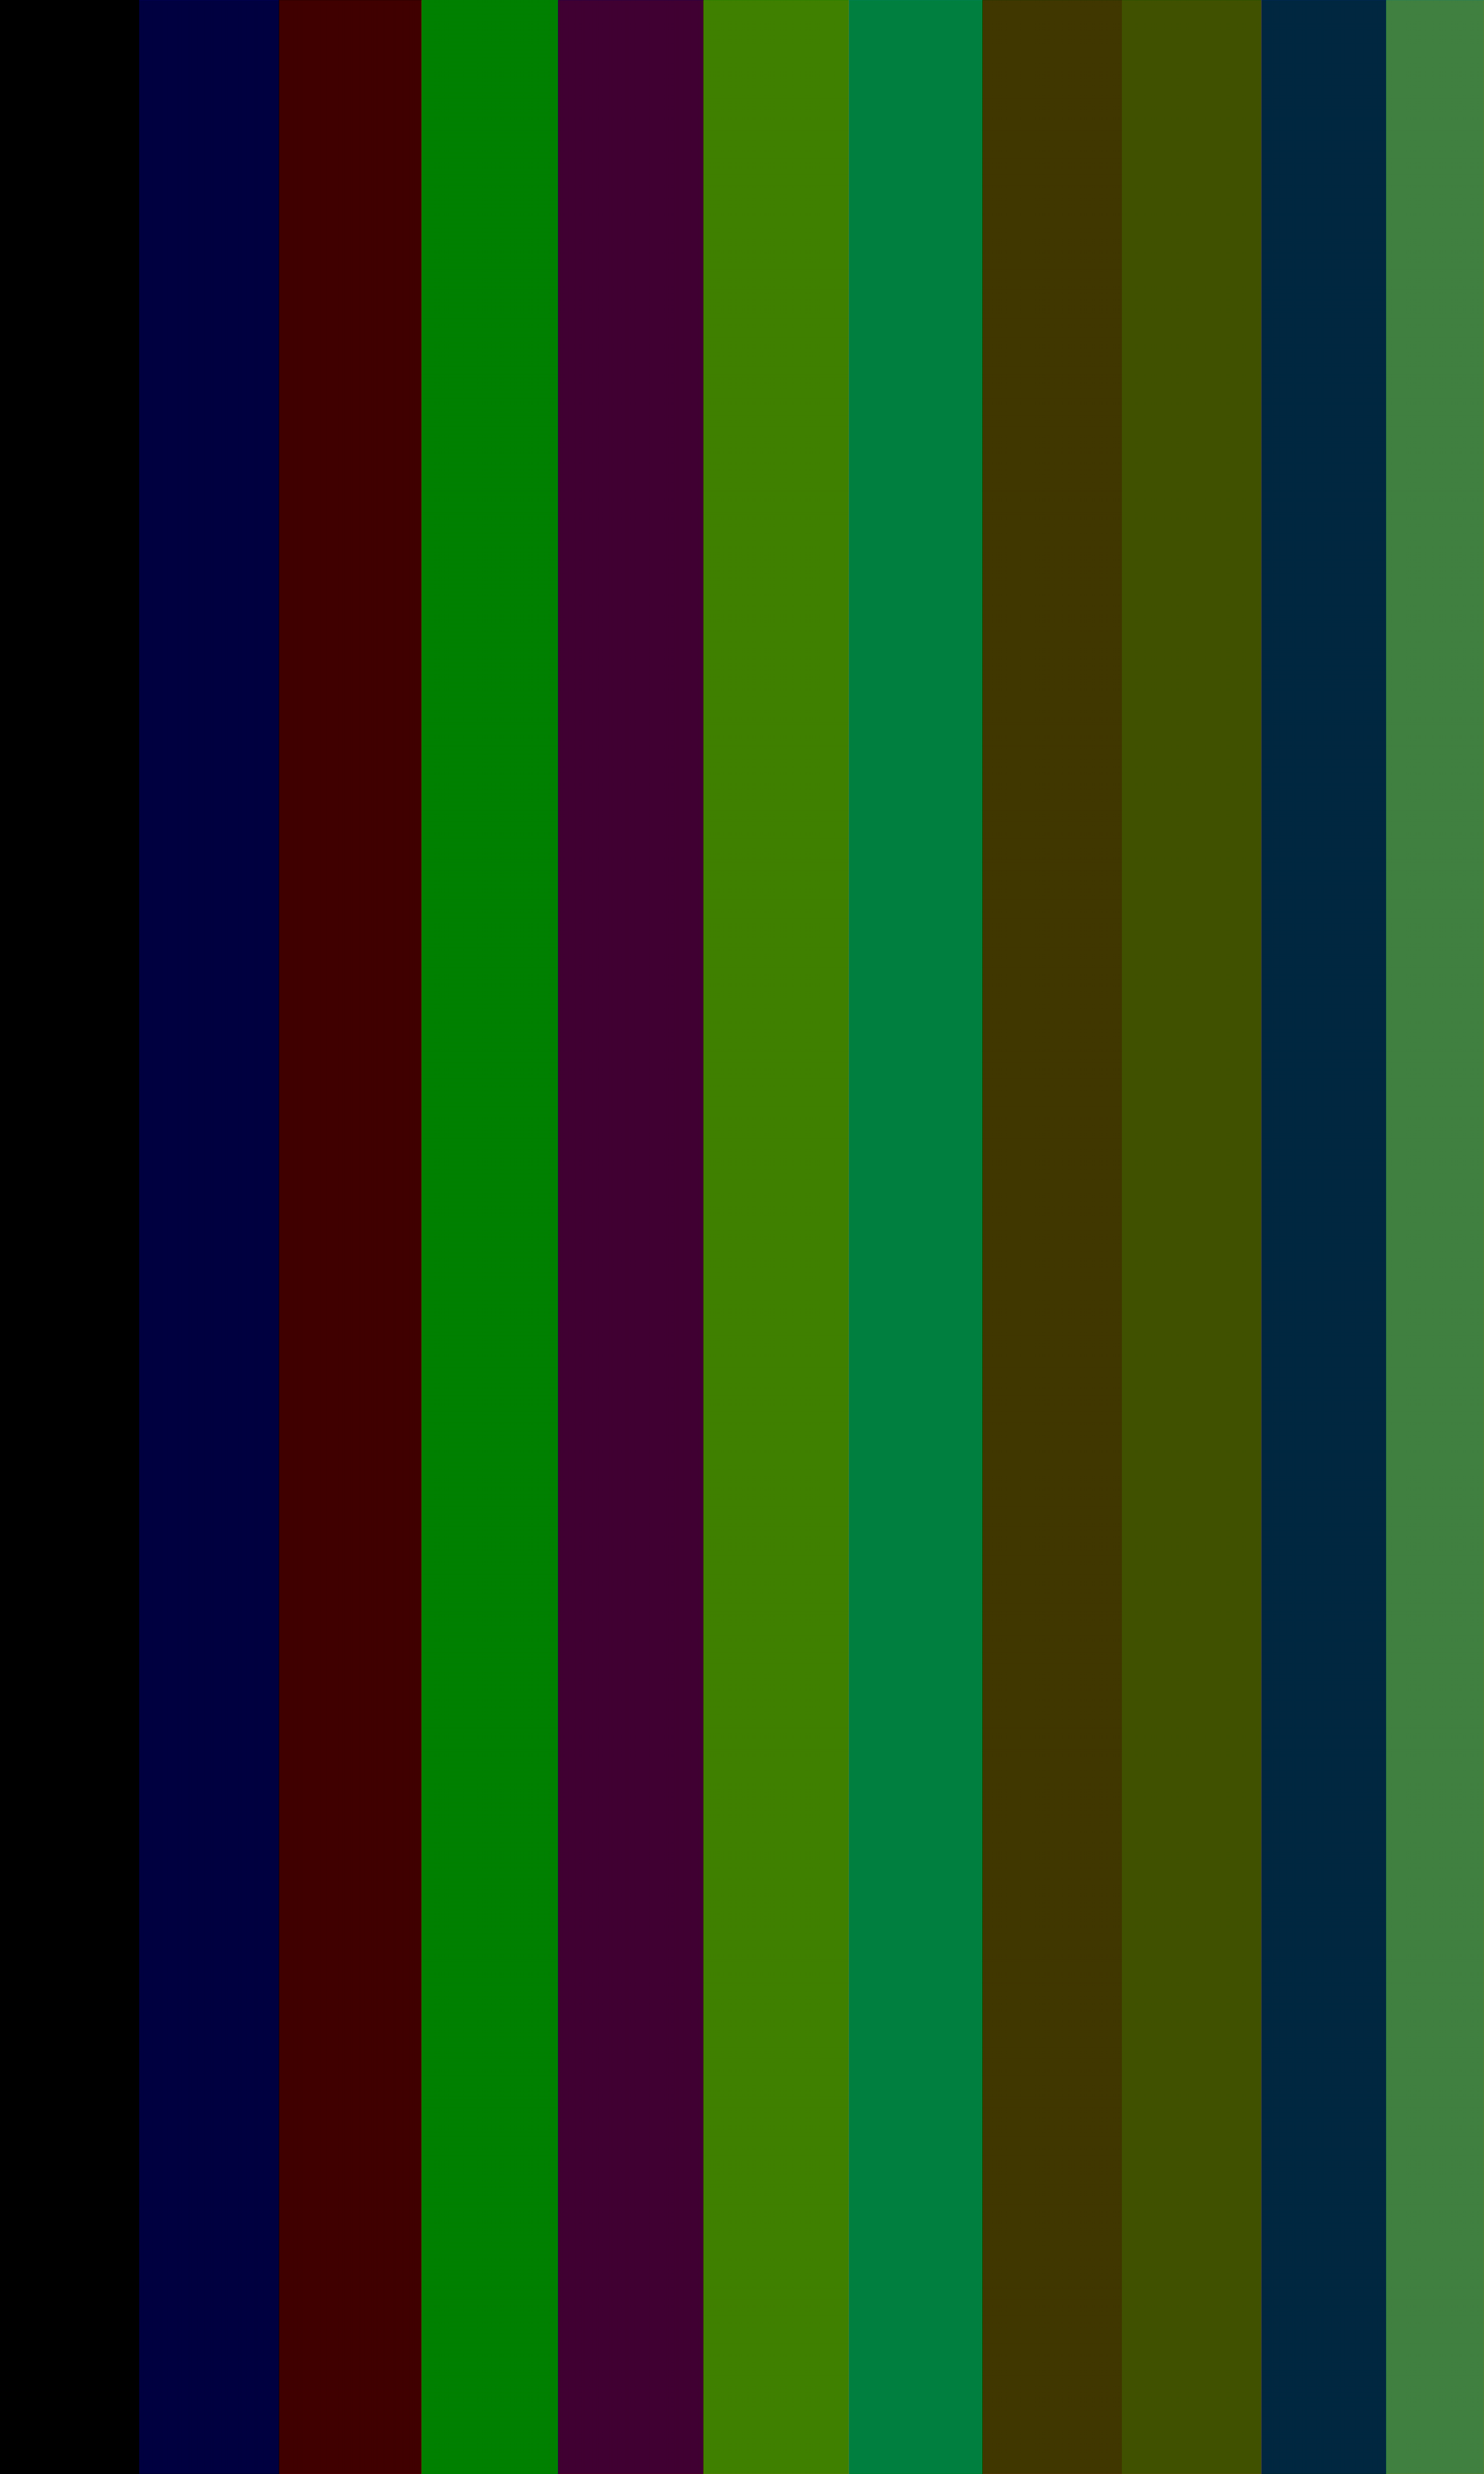
\includegraphics[scale=0.04]{imagenes/colores_bayer.png}
       \caption{Bayerizada}\label{fig:awesome_image1}
        \end{center}
\endminipage\hfill 
\end{figure}
\newpage
\begin{figure}[!htb]
\minipage{0.5\textwidth}
\begin{center}
    
\includegraphics[scale=0.04]{imagenes/colores_demosicing_bilineal.png}
    \caption{Bilineal }
 \end{center}
\endminipage
\minipage{0.5\textwidth}
\begin{center}
    
\includegraphics[scale=0.04]{imagenes/colores_demosicing_quality.png}
    \caption{High Quality}
        \end{center}
\endminipage\hfill
\end{figure}

\begin{figure}
\minipage{0.5\textwidth}
\begin{center}
    
\includegraphics[scale=0.04]{imagenes/colores_demosicing_spline.png}
    \caption{Directional}
        \end{center}
\endminipage
\minipage{0.5\textwidth}
\begin{center}
    
\includegraphics[scale=0.04]{imagenes/colores_demosicing_vecino.png}
    \caption{Vecinos}
 \end{center}
\endminipage
 
\end{figure}
\newpage

Efectivamente a primera vista parecería que todas dieran lo mismo. Pero veamos que si le hacemos zoom, no es así.
\begin{figure}[!htb]
\minipage{0.5\textwidth}
\begin{center}
    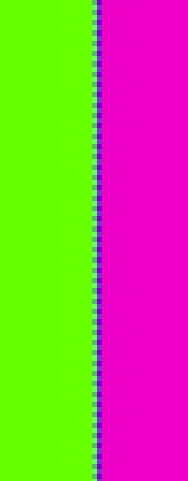
\includegraphics[scale=0.6]{imagenes/colores_bilineal_zoom.jpg}
    \caption{Bilineal Zoom}
        \end{center}
\endminipage
\minipage{0.5\textwidth}
\begin{center}
    
\includegraphics[scale=0.6]{imagenes/colores_hq_zoom.jpg}
    \caption{High Quality Zoom}
        \end{center}
\endminipage 
\end{figure}
\newpage
\begin{figure}[!htb]
\minipage{0.5\textwidth}
\begin{center}
    
\includegraphics[scale=0.6]{imagenes/colores_directional_zoom.jpg}
    \caption{Directional Zoom}
        \end{center}
\endminipage
\minipage{0.5\textwidth}
\begin{center}
    
\includegraphics[scale=0.6]{imagenes/colores_vecinos_zoom.jpg}
    \caption{Vecinos Zoom}
        \end{center}
\endminipage 
\end{figure}


El algoritmo bilineal y el high quality tuvieron pequeños errores en los bordes. Podemos observar que en esos casos entre el verde y el violeta parece haber como una `cosedura', la misma se repite en todos los bordes de la imagen. Estas diferencias imperceptibles por el tamaño de la imagen a primera vista pueden ser efectivamente comprobadas mediante un análisis de calidad objetivo. 

A continuación podemos ver los PSNR obtenidos al comparar los distintos resultados con la imagen original. Las im{ágenes que al hacerles zoom tenían esas $"$coseduras$"$ efectivamente fueron las que mas bajo PSNR dieron, es decir las que mas difirieron de la real.

$$ 
\begin{bmatrix}
           &      PSNR     \\
       highquality    &   39.67   \\
       bilineal    &      41.14   \\
       directional    &      48.13    \\
       vecinos   &      048.13      \\
\end{bmatrix} 
$$

A continuación veremos también cual fué el tiempo de computo de cada algoritmo.

$$ 
\begin{bmatrix}
           &      Tiempo (segundos)     \\
       highquality    &   64.88   \\
       bilineal    &      63.00   \\
       directional    &      57.82    \\
       vecinos   &      10.31      \\
\end{bmatrix} 
$$

Como era de esperarse, las proporc1iones tiempo tienen sentido. Vecinos es el mas rápido ya que es el procedimiento mas simple y quality tarda mas que bilineal ya que antes aplica bilineal para luego mejorarlo (aunque en este caso no lo mejora). Para este caso tanto por calidad objetiva, subjetiva como en tiempo de cómputo vecinos parecería ser el mejor.


\newpage

\subsection{Imagen 9 - Avión}

Nos pareció interesante hacer un análisis particular de la Imagen 9 ya que posee varias características en donde se pueden observar diferentes condiciones para ver como actúan los cuatro algoritmos, estos son: tener gran cantidad de sectores bordes, gran variedad de colores que contrastan altamente y principalmente tener texto. Destacamos esto último ya que una de las cualidades más importantes que deben poseer estos algoritmos es la de asegurar nitidez y suavidad, detalles que se ven al procesar imágenes que poseen texto. \\
A continuación mostraremos el resultado de los algoritmos para esta imagen:

\begin{figure}[h]
       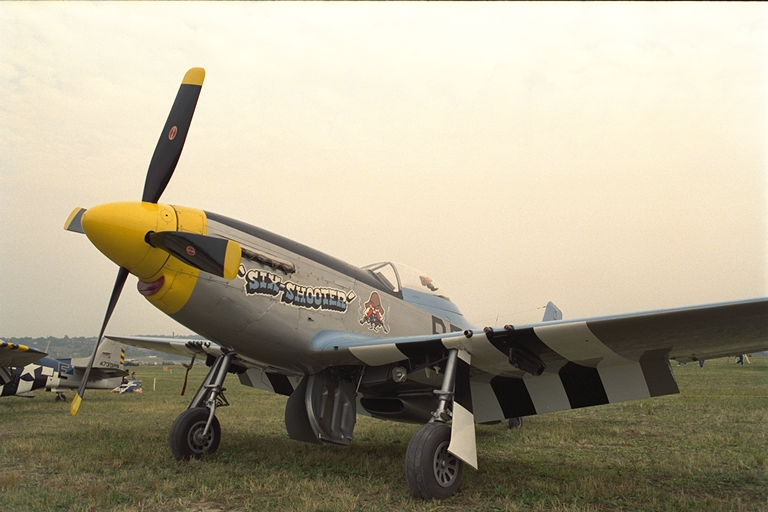
\includegraphics[width=0.5\textwidth]{imagenes/img9.png}
           \hfill
        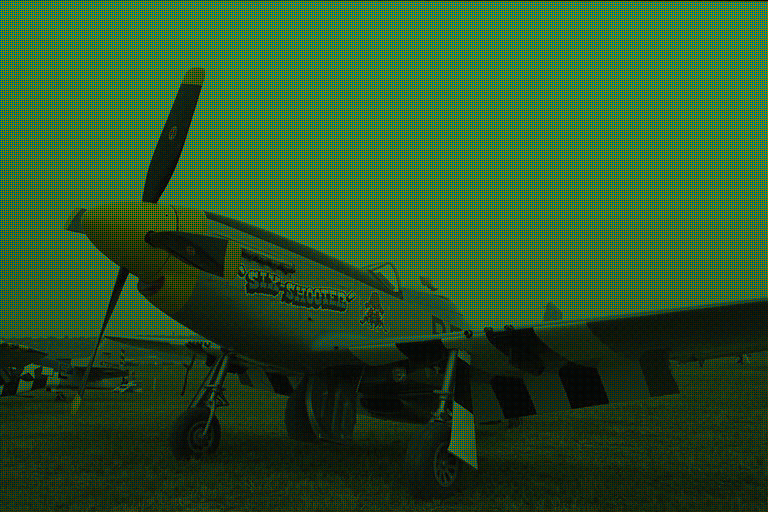
\includegraphics[width=0.5\textwidth]{imagenes/img9_bayer.png}   
        Imagen original y bayerizada
\end{figure}

\begin{figure}[h]
       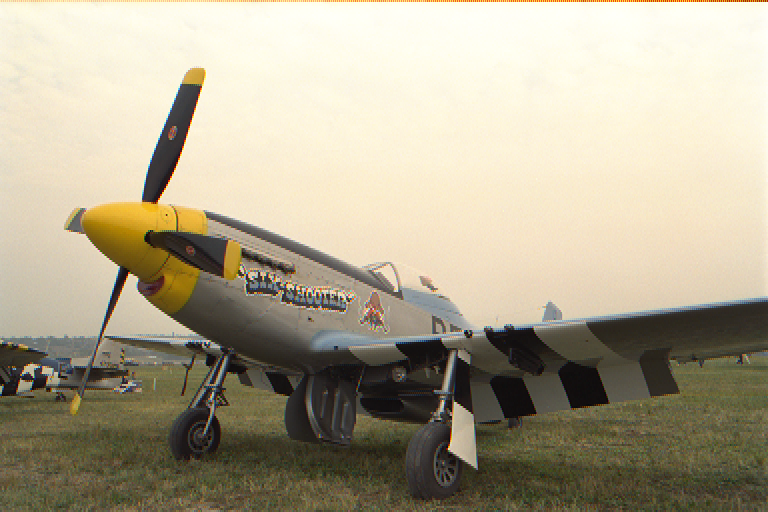
\includegraphics[width=0.5\textwidth]{imagenes/img9_demosicing_vecino.png}
           \hfill
        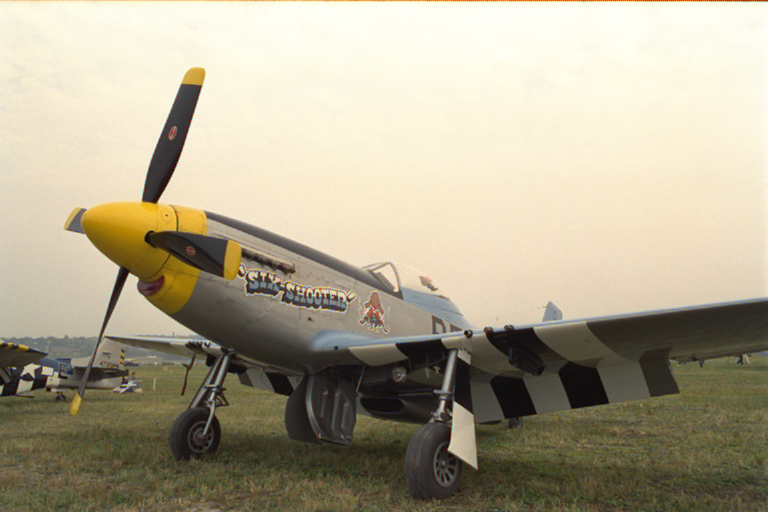
\includegraphics[width=0.5\textwidth]{imagenes/img9_demosicing_bilineal.png}
        Algoritmos de Vecinos e Interpolación Bilineal
\end{figure}


\begin{figure}[h]
       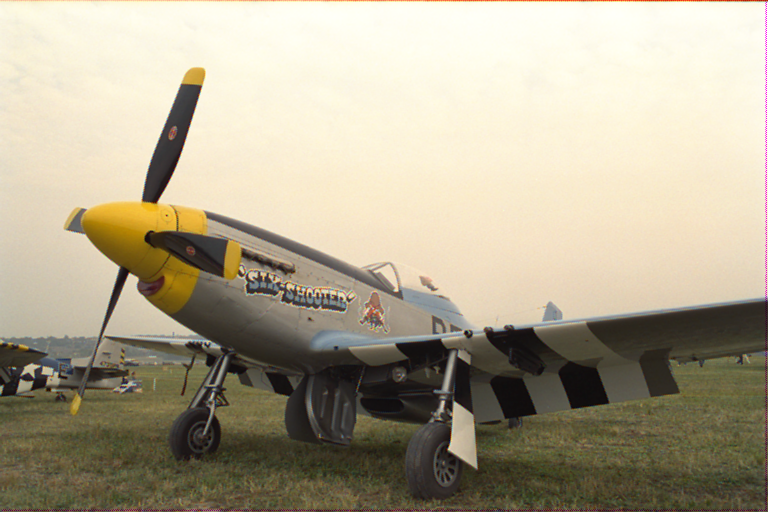
\includegraphics[width=0.5\textwidth]{imagenes/img9_demosicing_spline.png}
           \hfill
        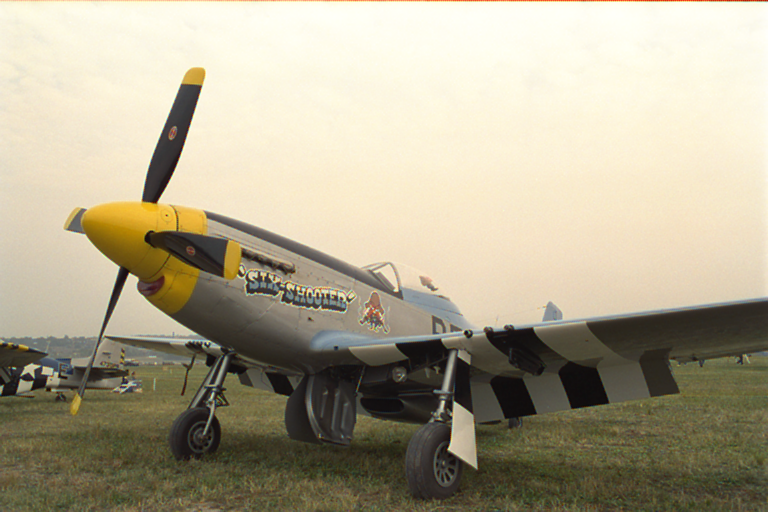
\includegraphics[width=0.5\textwidth]{imagenes/img9_demosicing_quality.png}
        Algoritmos de Interpolación Direccional y HighQuality
\end{figure}
\newpage

Como se puede observar, a simple vista pareciera que los 4 algoritmos dan un resultado bastante aceptable, pero mirando detalladamente y comparando entre sí se puede observar una gran diferencia entre ellos, principalmente en zonas borde y en la zona del texto del avión. Subjetivamente pareciera ser que la imagen más parecida a la original es la del HighQuality, seguida por la Interpolación Direccional, pero objetivamente en base a los resultados obtenidos al método PSNR se observa que el algoritmo de Interpolación Bilineal supera al Direccional, algo que llama bastante la atención y que indica que lo subjetivo se diferencia bastante de los objetivo. 

$$ 
\begin{bmatrix}
        algoritmo   &      PSNR     \\
       highquality    &   37.71  \\
       bilineal    &     35.34  \\
       directional    &      33.35    \\
       vecinos   &      30.49     \\
\end{bmatrix} 
$$
Yendo más a fondo aún en la cuestión y para mostrar el nivel de detalle que obtiene cada algoritmo, decidimos hacer zoom en la zona donde la imagen posee texto:

\begin{figure}
       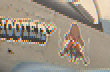
\includegraphics[width=0.5\textwidth]{imagenes/img9_demosicing_vecino_cropped.png}
        \caption{Vecinos}
\end{figure}

\begin{figure}
       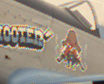
\includegraphics[width=0.5\textwidth]{imagenes/img9_demosicing_bilineal_cropped.png}
        \caption{Bilineal}
\end{figure}

\begin{figure}
       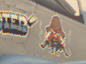
\includegraphics[width=0.5\textwidth]{imagenes/img9_demosicing_spline_cropped.png}
        \caption{Direccional}
\end{figure}

\begin{figure}
       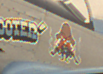
\includegraphics[width=0.5\textwidth]{imagenes/img9_demosicing_quality_cropped.png}
        \caption{Quality}
\end{figure}

Acá si se puede observar la nitidez y suavidad que presenta cada algoritmo, viéndose como mejora la calidad del texto para cada imagen y como va disminuyendo el ruido aumentando la refinación alrededor del mismo.

\newpage

\subsection{Imagen 12}

A continuación probaremos con una imagen provista por la cátedra para tener mas resultados sobre los cuales apoyarnos a la hora de sacar nuestras conclusiones. Obviaremos la imagen bayerizada ya que sólo
nos interesaba ver que sea correcta la bayerización y con lo ya hecho eso queda claro.

\begin{figure}[h]
\begin{center}
       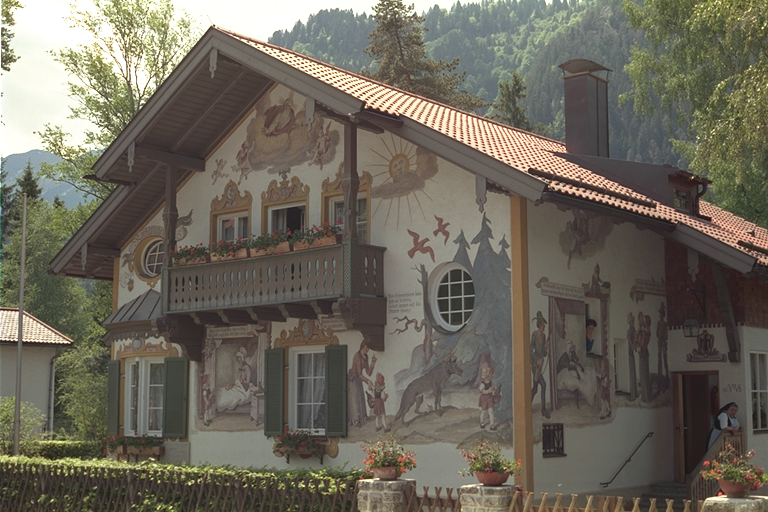
\includegraphics[scale=0.3]{imagenes/img12.png}
       \caption{Original }\label{fig:awesome_image1}
        \end{center}

\end{figure}

\begin{figure}[!ht]
\minipage{0.5\textwidth}
\begin{center}
    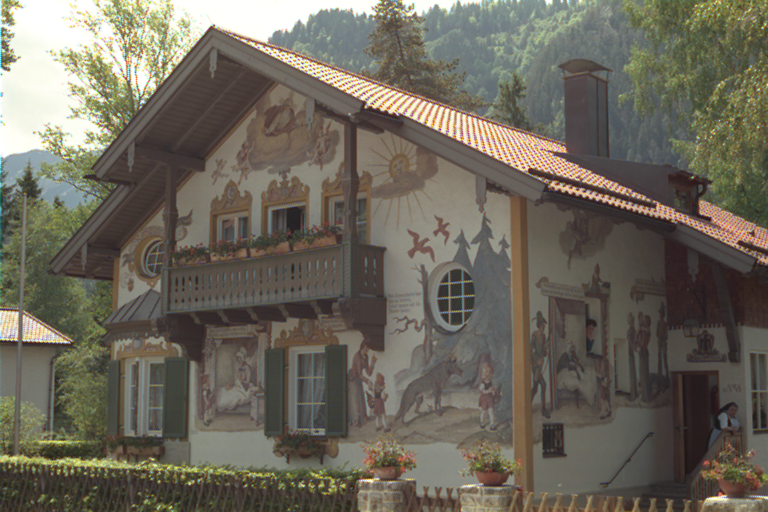
\includegraphics[scale=0.3]{imagenes/img12_demosicing_bilineal.png}
    \caption{Bilineal }
 \end{center}
\endminipage
\minipage{0.5\textwidth}
\begin{center}
    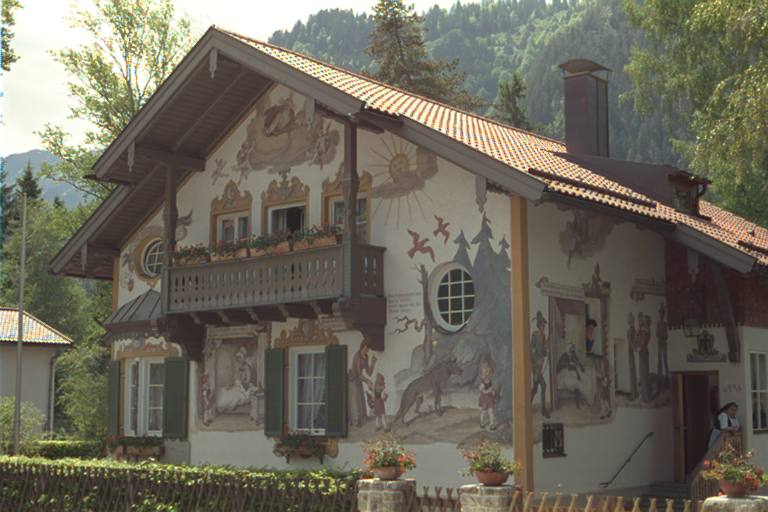
\includegraphics[scale=0.3]{imagenes/img12_demosicing_quality.png}
    \caption{High Quality}
        \end{center}
\endminipage\hfill
\end{figure}

\begin{figure}[h]
\minipage{0.5\textwidth}
\begin{center}
    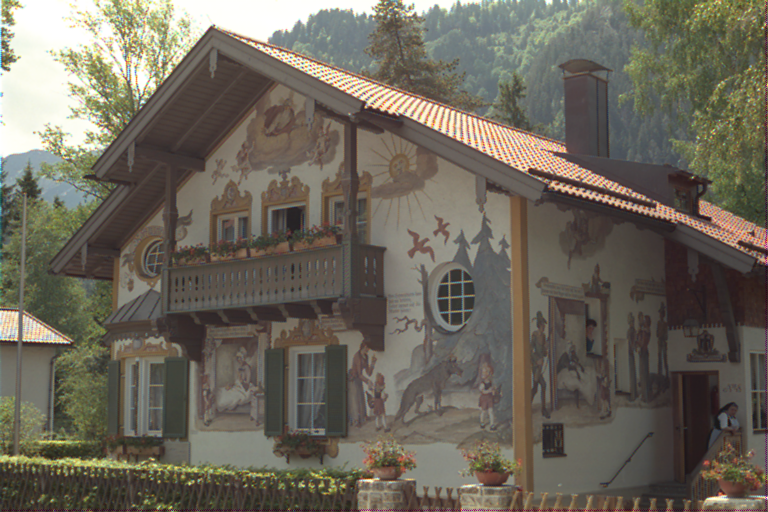
\includegraphics[scale=0.3]{imagenes/img12_demosicing_spline.png}
    \caption{Directional}
        \end{center}
\endminipage
\minipage{0.5\textwidth}
\begin{center}
    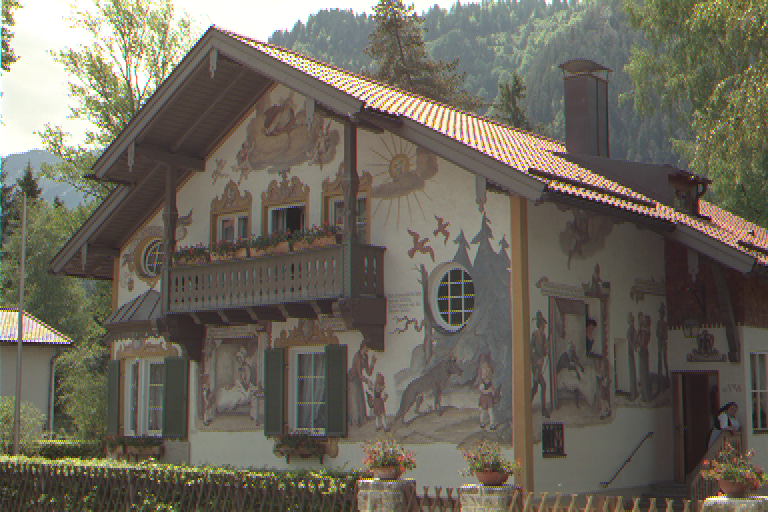
\includegraphics[scale=0.3]{imagenes/img12_demosicing_vecino.png}
    \caption{Vecinos}
 \end{center}
\endminipage
 
\end{figure}
\newpage

Subjetivamente highquality parece ser la mejor. Ya que se la ve bastante menos borrosa que las demás y con bordes mas nítidos, esto es facilmente apreciable en los dibujos que hay sobre la casa. A diferencia de vecinos que tiene bordes no sólo poco nítidos sino hasta claramente pixelados. Entre Directional y bilineal podemos notar que el primero, en los dibujos de la casa, es un poco más nitido que el segundo y parece tener un poco mas de calidad, también apreciable en los dibujos de la casa.

Veamos ahora a través del calculo del PSNR contra la imagen original como es el ranking.

$$ 
\begin{bmatrix}
           &      PSNR    \\
       quality    &   32.33   \\
       bilineal    &      30.27   \\
       directional    &      29.87    \\
       vecinos   &      25.45     \\
\end{bmatrix} 
$$

Objetivamente el peor y el mejor se mantienen, debido a que quality es el de mayor PSNR y vecinos el de menor. En estos valores también es apreciable la gran diferencia de resultados observada anteriormente, mientras que subjetivamente se podía notar una nítida y la otra directamente pixelada objetivamente el PSNR es 10 puntos mas grande en la quality. Lo que si cambia acá es la relación entre directional y bilineal, mientras que objetivamente el bilineal parecía ser mejor subjetivamente podemos ver que esto es al revés (aunque también por poca diferencia).

Como dato interesante vale aclarar que en el tejado de la casa podemos ver anomalías en todos los resultados, así como también en los arboles que estan a la izquierda y por encima. Más adelante analizaremos bien porque es que sucede esto.


\newpage

\subsection{Calidad subjetiva}

